\section{Results}
%-------------------------------------------------
\begin{frame}{Results - Centralities}
	\begin{itemize}
		\item determine the relative importance of a vertex within a graph
		\item centraltity concepts were first developed in social network analysis
		\begin{description}
			\item[-->] e.g. how influential a person is within a social network
		\end{description}
	\end{itemize}
	
	\begin{definition}[Four measures of centrality]
		\begin{enumerate}
			\item degree centrality
			\item eccentricity centrality			
			\item closeness centrality
			\item betweeness centrality
		\end{enumerate}
	\end{definition}
\end{frame}
%-------------------------------------------------
\begin{frame}{Results - Degree Centrality}
	\begin{definition}[Degree Centrality]
		$C_{deg}(v) = \{e|e \in E\; and\; v \in e\}$
	\end{definition}
	\begin{itemize}
		\item counts the number of edges attached to a vertex
		\item a local centrality measure
		\begin{description}
			\item[-->] only direct neighborhood considered 
		\end{description}
		\item directed graphs:
		\begin{description}
			\item[-->] indegree (interpreted as "popularity")
			\item[-->] outdegree (interpreted as "gregariousness")
		\end{description}
	\end{itemize}
\end{frame}
%-------------------------------------------------
\begin{frame}{Results - Degree Centrality}
\begin{figure}
	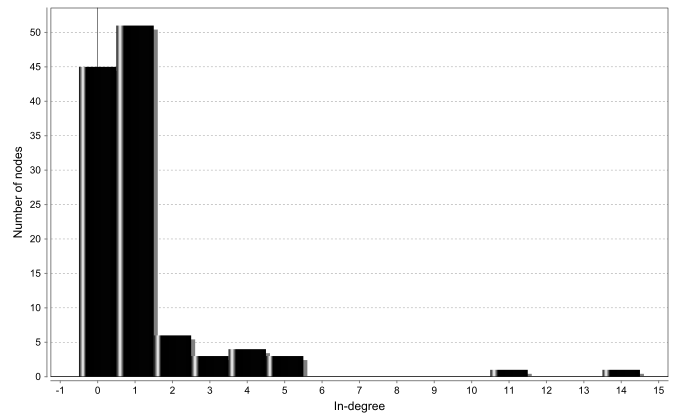
\includegraphics[scale=0.4]{inc/img/Glyco1/InDegreeDistr.png}
%\subfigure[Glyco1]{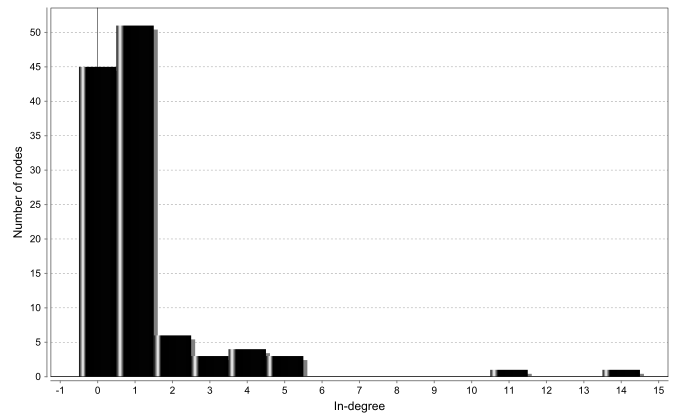
\includegraphics[scale=0.25]{inc/img/Glyco1/InDegreeDistr.png}}\hfill
%\subfigure[Glyco2]{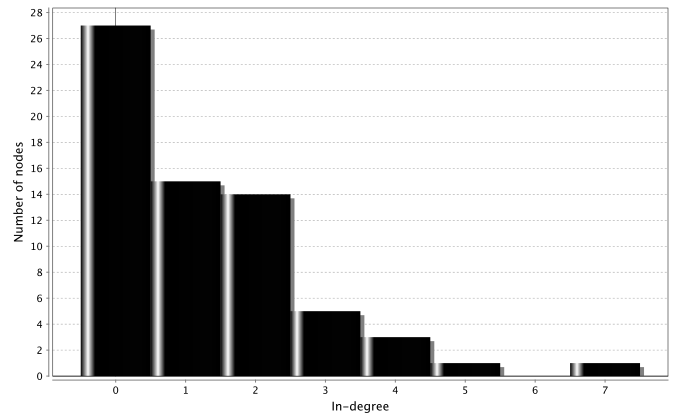
\includegraphics[scale=0.25]{inc/img/Glyco2/InDegree.png}}
\caption{Indegree Centrality}
\end{figure}
\end{frame}
%-------------------------------------------------
\begin{frame}{Results - Degree Centrality}
\begin{figure}
	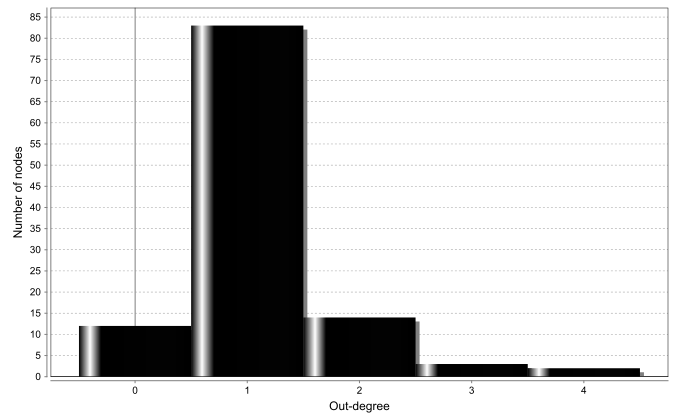
\includegraphics[scale=0.4]{inc/img/Glyco1/OutDegreeDistr.png}
%\subfigure[Glyco1]{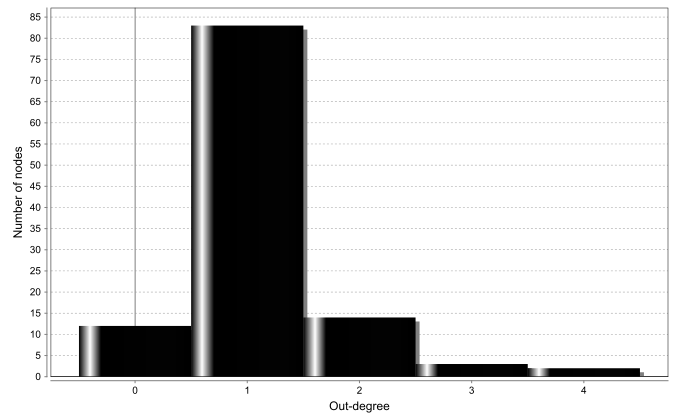
\includegraphics[scale=0.25]{inc/img/Glyco1/OutDegreeDistr.png}}\hfill
%\subfigure[Glyco2]{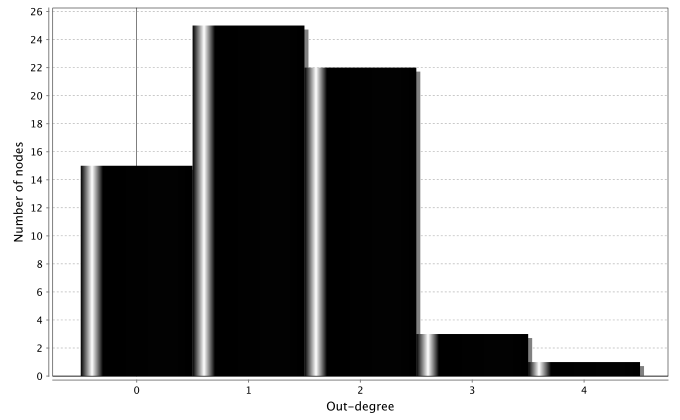
\includegraphics[scale=0.25]{inc/img/Glyco2/OutDegree.png}}
\caption{Outdegree Centrality}
\end{figure}
\end{frame}
%-------------------------------------------------
\begin{frame}{Results - Eccentricity Centrality}
	\begin{definition}[Eccentricity Centrality]
		$C_{ecc}(s) = \frac{1}{max\{d_{st}|t\in V\}}$
	\end{definition}
	\begin{itemize}
		\item determine the maximum distance between every two vertices
		\item central vertices get low values
		\item centralities require high centrality values
		\begin{description}
			\item[-->] reciprocal is used as centrality value
		\end{description}
		\item only for CONNECTED networks
	\end{itemize}
\end{frame}
%-------------------------------------------------
\begin{frame}{Results - Eccentricity Centrality}
	\begin{figure}
		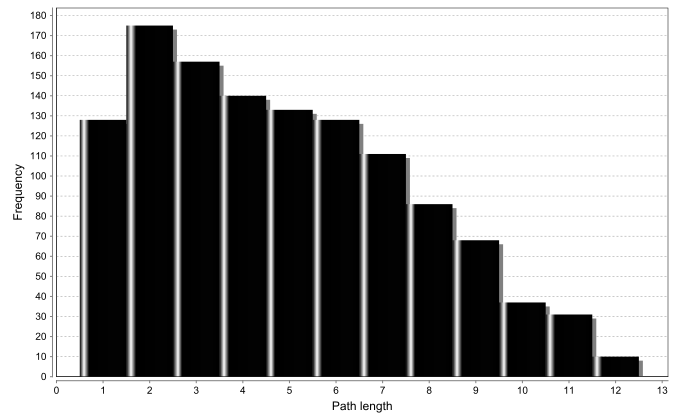
\includegraphics[scale=0.4]{inc/img/Glyco1/ShortPathLengthDistr.png}
	%\subfigure[Glyco1]{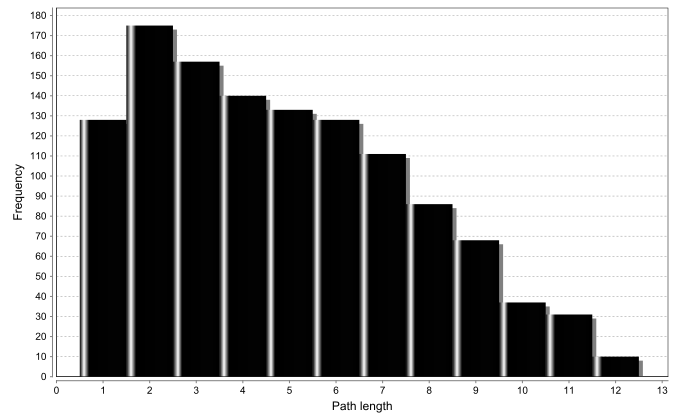
\includegraphics[scale=0.25]{inc/img/Glyco1/ShortPathLengthDistr.png}}\hfill
	%\subfigure[Glyco2]{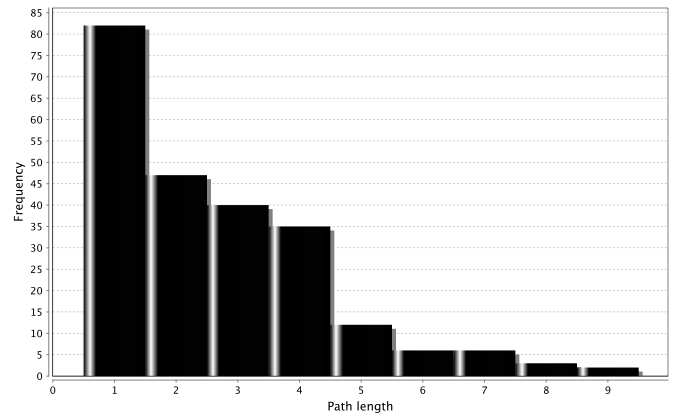
\includegraphics[scale=0.25]{inc/img/Glyco2/ShortestPathLengthDistr.png}}
	\caption{Eccentricity Centrality}
	\end{figure}
\end{frame}
%-------------------------------------------------
\begin{frame}{Results - Closeness Centrality}
	\begin{definition}[Closeness Centrality]
		$C_{clo}(s) = \frac{1}{\sum\limits_{t\in V} d_{st}}$
	\end{definition}
	\begin{itemize}
		\item $C_{clo}$ of a vertex s is the sum of shortest path form s to all other vertices  
		\item degree of interaction in the network
		\item the closer a point is to all the rest, the more effective and independent he can reach them
	\end{itemize}
\end{frame}
%-------------------------------------------------
\begin{frame}{Results - Closeness Centrality}
	\begin{figure}
		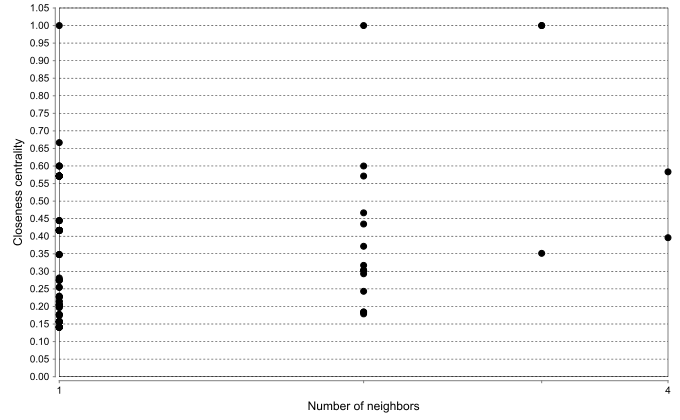
\includegraphics[scale=0.4]{inc/img/Glyco1/ClosenessCentr.png}
	%\subfigure[Glyco1]{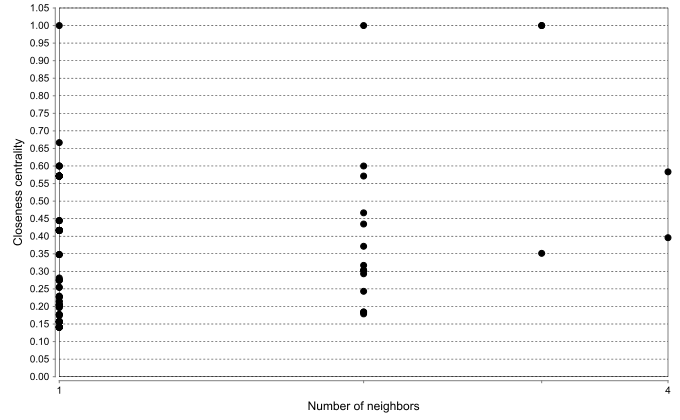
\includegraphics[scale=0.25]{inc/img/Glyco1/ClosenessCentr.png}}\hfill
	%\subfigure[Glyco2]{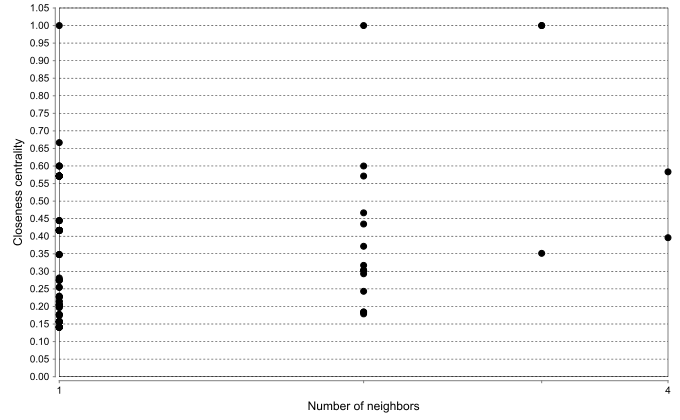
\includegraphics[scale=0.25]{inc/img/Glyco1/ClosenessCentr.png}} %TODO hier noch für Glyco 2 einbinden
	\caption{Closeness Centrality}
	\end{figure}
\end{frame}
%-------------------------------------------------
\begin{frame}{Results - Betweenness Centrality}
	\begin{definition}[Betweenness Centrality]
		$C_{spb}(v)=\sum\limits_{s \in V\; and\; s \neq v} \sum\limits_{t \in V\; and\; s \neq v} \delta_{st}(v)$
	\end{definition}
	\begin{itemize}
		\item center of attention: indirect relationships 
		\begin{description}
			\item[-->] Control of interaction
		\end{description}
		\item v is the more powerful the more shortest paths between other vertices it can interrupt
	\end{itemize}
\end{frame}
%-------------------------------------------------
\begin{frame}{Results - Betweenness Centrality}
	\begin{figure}
		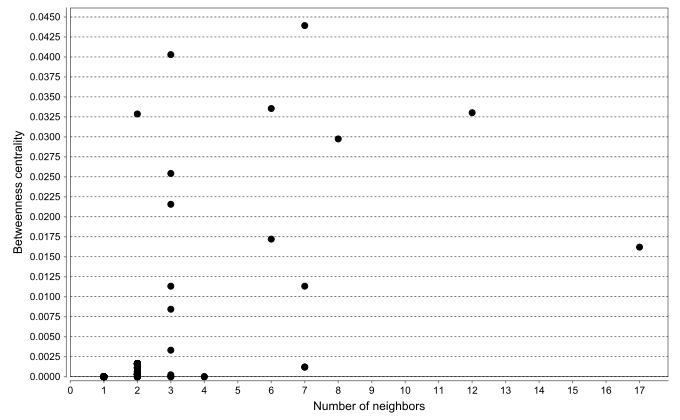
\includegraphics[scale=0.4]{inc/img/Glyco1/BetweennessCentr.png}
	%\subfigure[Glyco1]{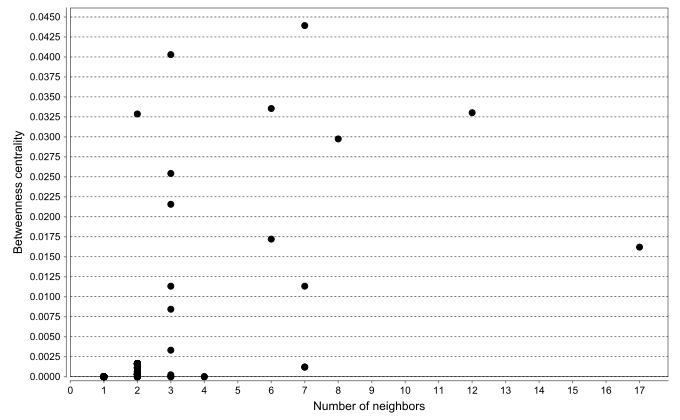
\includegraphics[scale=0.25]{inc/img/Glyco1/BetweennessCentr.png}}\hfill
	%\subfigure[Glyco2]{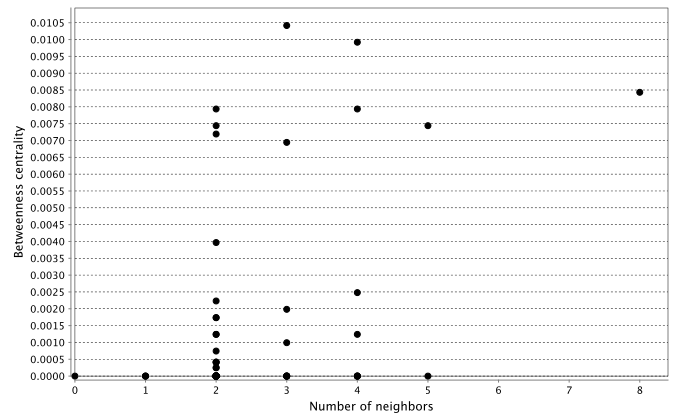
\includegraphics[scale=0.25]{inc/img/Glyco2/BetweennessCentr.png}}
	\caption{Closeness Centrality}
	\end{figure}
\end{frame}
%-------------------------------------------------
\begin{frame}{Results - Conclusion}
	\begin{itemize}
		\item the analysis tools are not very helpful
		\begin{description}
			\item[-->] cannot see which vertex has which centrality
			\item[-->] only give a statistical overview of the whole network
		\end{description}
		\item \textbf{but} you can select a vertex in the network window and get an overview of all centralities from the selected vertex
	\end{itemize}
\end{frame}
%-------------------------------------------------
\begin{frame}{Results - Conclusion}
	\begin{figure}
		\includegraphics[scale=0.35]{inc/img/Glyco1/Vertex_Centricities.PNG}
	%\subfigure[Glyco1]{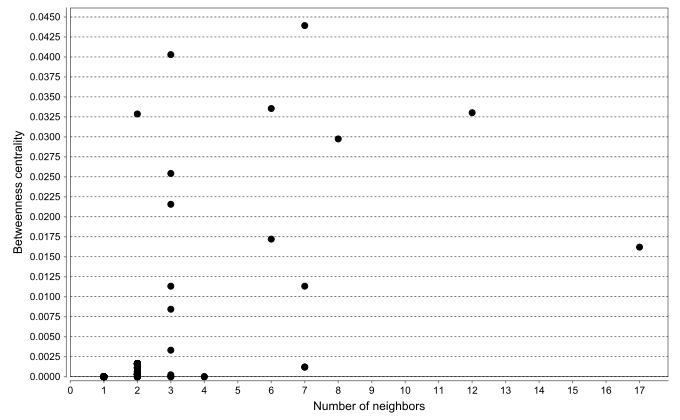
\includegraphics[scale=0.25]{inc/img/Glyco1/BetweennessCentr.png}}\hfill
	%\subfigure[Glyco2]{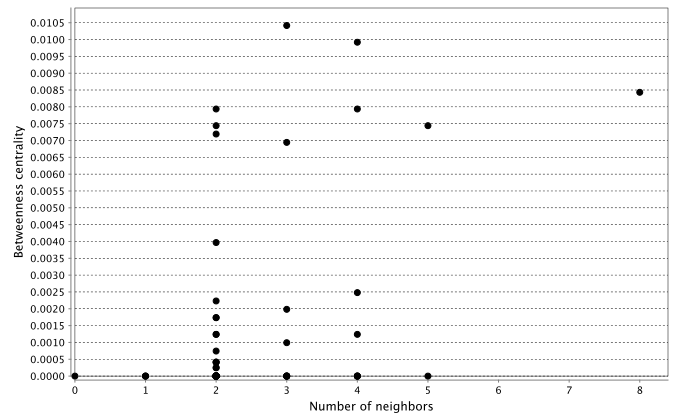
\includegraphics[scale=0.25]{inc/img/Glyco2/BetweennessCentr.png}}
	\caption{Centrality Overview}
	\end{figure}
\end{frame}